

\section{Project organization}
We decided to use the scrum model for organizing our group. This means that we have a flat organizational structure where everyone contributes with what they are able to. Even in a flat structure, it is important to share responsibilities, so each person of the group got responsibility of a main focus area. If it becomes too much work for one person, we have decided that it is important that the work is delegated to the others.

\subsection{Organizational diagram}
See figure \ref{fig:organizationalchart} below for an organizational diagram that shows the internal structure of our group, as well as our connection to our advisor and Thales. Notice that even though we have a project leader, he is at the same level as all the others. This is to indicate that the project leader is not a big boss, but that we are all equally responsible for this project being a success.
\begin{figure}[hbt]
\begin{center}
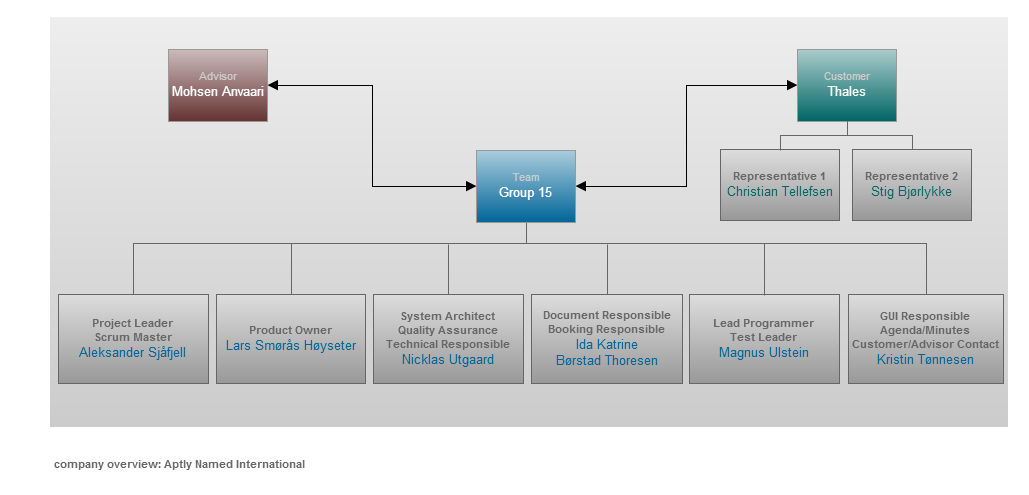
\includegraphics[width=\textwidth]{Organizational_Chart_v2}
\caption{Organizational chart} \label{fig:organizationalchart}
\end{center}
\end{figure}

\newpage

\subsection{Role allocation}
See table \ref{tab:roleallocation} below for a role allocation table that shows what roles each person was assigned, as well as a short description of the role. The roles is merely a guideline on who are responsible for the depicted area. If the person would need more help, then we have all agreed to contribute to get the result we want. We are all in this together.
\begin{table}[h!]
\begin{center}
\begin{tabularx}{\linewidth}{>{\setlength\hsize{.5\hsize}}X|>{\setlength\hsize{0.3\hsize}}X|>{\setlength\hsize{1\hsize}}X} \hline
\textbf{Role} & \textbf{Person} & \textbf{Responsibilities} \\ \hline \hline

Project leader & Aleksander & Make sure everybody does what they are supposed to and peacefully resolve disputes between participants \\  \hline
Scrum master & Aleksander & Make sure the team’s work conform to Scum standards and help the team do the best work possible \\ \hline

Booking of rooms & Ida & Booking rooms for the meetings and other activities \\ \hline
Document responsible & Ida &Keep track of what is to be contained in the project report, what has been written and what remains \\ \hline
Project report layout responsible & Ida &Find software to make tables and graphs, and check that all diagrams are similar in style \\ \hline

Responsible for graphical user interface & Kristin & Design the views and the interactions and setting up the MVC structure \\ \hline
Agendas, minutes of meetings & Kristin &Write agendas and minutes of meeting and send these out within the specified time limits \\ \hline
Customer/advisor contact & Kristin & Main contact person for customer and advisor \\ \hline

Product owner & Lars & Represent the stakeholders and ensure that the team delivers value to business\\ \hline

Test leader & Magnus & Lead the testing team \\ \hline
Lead programmer & Magnus & Responsible for having a general overview of the code. This means knowing what is to be implemented next, and seeing that this is done at the right time \\ \hline

System architect & Nicklas & Defining the system architecture \\ \hline
Technical responsible & Nicklas & Setup of Netbeans, Git and other tools that the team uses in the development \\ \hline
Quality assurance responsible & Nicklas & Make sure that all routines, templates and standards are followed \\ \hline

\end{tabularx}
\end{center}
\caption {Role allocation} \label{tab:roleallocation}
\end{table}

\newpage

\subsection{Weekly schedule}
See table \ref{tab:weeklyschedule} below for a weekly schedule that shows how we have allocated time for the Customer Driven Project. As we all have said how much we are able to contribute to the project, we have agreed to ensure that work outside of group work-hours must be done to reach the goal.
\begin{table}[h!]
\begin{center}
\begin{tabular}{l|l|l|l|l|l} \hline
 & \textbf{Monday} & \textbf{Tuesday} & \textbf{Wednesday} & \textbf{Thursday} & \textbf{Friday} \\ \hline \hline
\textbf{08-09} &  & Group work &  &  &  \\
\textbf{09-10} &  & Group work &  &  &  \\
\textbf{10-11} &  & Group work &  &  &  \\
\textbf{11-12} &  & Advisor meeting & &  &  \\
\textbf{12-13} & Group work & Group work & Customer meeting &  &  \\
\textbf{13-14} & Group work & Group work & Group work &  &  \\
\textbf{14-15} & Group work & Group work & Group work &  &  \\
\textbf{15-16} & Group work &  & Group work &  &  \\
\textbf{16-17} & Group work &  & Group work &  &  \\
\textbf{17-18} & Group work &  & Group work &  & \\ \hline
\end{tabular}
\end{center}
\caption {Weekly schedule} \label{tab:weeklyschedule}
\end{table}


